\section{Literature Review and Technical Rationale}

This chapter employs the literature review as a design rationale rather than a mere repetition of the implementation details. It specifically addresses how existing research justifies the technical choices made in this thesis regarding Mie-based geometric observables, short-pulse penetration behaviour, multihole plume registration, right-censored targets, uncertainty-aware surrogate modelling, and probabilistic impingement screening, while identifying gaps that are not fully covered by any single strand of literature. The objective is to explicitly establish a logical chain from prior knowledge to engineering design decisions before the workflow itself is described.
\subsection{Introduction to Methodological Terminology for Interdisciplinary Readers}\label{sec:methods-terminology}

The implementation of this thesis spans four technical domains: 
computer vision, numerical optimization, GPU parallel computing, and deep learning. 
These four tools are sequentially integrated in this work: 
image processing extracts penetration observables from videos; 
robust optimization compresses noisy trajectories into stable fitting targets; 
GPU parallelism allows large-batch processing to be completed within a reasonable timeframe; 
and neural networks learn conditional predictive distributions from these targets. 
For readers whose primary background is in fluid mechanics and mechanical design, 
this section first provides an intuitive explanation of the minimum necessary concepts 
in each domain, 
so that the technical choices in subsequent sections can be understood 
as engineering decisions rather than inscrutable black boxes.

\textbf{Computer Vision and Signal Processing.}
Computers store images as numerical matrices: 
each pixel corresponds to an element in the matrix, 
with its value representing the intensity or brightness at that point. 
Processing an image essentially means applying mathematical operations to this matrix. 
\emph{Convolution} is the most fundamental operation: 
a small template window (convolution kernel) slides over the image pixel by pixel, 
performing a weighted sum at each step. 
Its effect depends on the shape of the kernel, 
allowing it to smooth the image, extract edges, or enhance textures. 
The Sobel operator is a convolution kernel that calculates local brightness gradients 
(rates of change); 
it responds most strongly to abrupt contrast changes such as liquid phase boundaries, 
making it a standard tool for locating boundaries in spray images. 
\emph{Polar coordinate transformation} converts an image from Cartesian coordinates 
(pixel rows and columns) into a coordinate system with angle and radial distance as axes. 
Performing this transformation around the calibrated nozzle center 
can fold the directional structure of a multi-hole spray into a 1D angular signal, 
greatly simplifying subsequent registration. 
The \emph{Fast Fourier Transform} (FFT) decomposes a signal into sinusoidal components 
of different frequencies, 
directly exposing periodic structures as frequency-domain peaks; 
this thesis uses it to automatically identify the rotational periodicity of multi-hole sprays, 
thereby estimating the angular offset of each hole.

\textbf{Robust Optimization and Curve Fitting.}
The geometric meaning of least squares fitting is to find a curve that minimizes 
the sum of squared distances from all observation points to that curve. 
When the data contains a small number of outliers 
(e.g., frames corrupted by optical noise or contains minor quantization error), 
the squared penalty allows these points to disproportionately affect the result. 
The Huber loss is a compromise: 
it retains the smoothness of the squared penalty when the residual is small, 
but switches to an absolute value penalty when the residual exceeds a threshold, 
thereby suppressing the leverage of outliers
---this is completely analogous to the engineering intuition of discarding anomalous readings 
in measurement practice. 
The \emph{gradient descent} algorithm used for neural network training calculates 
the partial derivative of the loss with respect to each parameter at the current parameter values, 
and then fine-tunes the parameters along the direction of steepest descent, 
repeating until the loss no longer decreases significantly
---conceptually equivalent to iteratively "walking downhill" in a high-dimensional parameter space.

\textbf{GPU Parallel Computing.}
CPUs typically have a few highly optimized cores that excel at processing complex, 
sequential logical tasks. 
GPUs have thousands of simpler cores, 
making them ideal for simultaneously applying the same arithmetic operations to a large number 
of well-organised data elements. 
Image processing perfectly fits this pattern: 
convolving each pixel, accumulating in each angular bin, thresholding each frame
---these operations are completely independent across pixels or frames, 
and the GPU can distribute them truly in parallel to thousands of cores for simultaneous execution. 
CUDA is a parallel computing platform provided by NVIDIA; 
CuPy is a Python library compatible with the NumPy interface, 
allowing the image processing chain in this thesis to switch to a GPU backend 
with minimal code changes. 
The engineering significance of GPU acceleration is transforming the batch processing of 
a terabyte-scale video archive from "taking several days" to "completing within a few hours and supporting iterative refinement", enabling the entire research workflow to be genuinely cyclical.

\textbf{Neural Networks and Deep Learning.}
The Multilayer Perceptron (MLP) is the type of neural network used in this thesis: 
several layers of linear transformations and non-linear activation functions are cascaded 
to form a non-linear function with tunable parameters, 
taking operating condition features and time as inputs, 
and outputting penetration predictions. 
The parameters are obtained through training
---repeatedly calculating the prediction error on a large number of samples 
and iteratively updating the weights using gradient descent until the overall error converges. 
Mean Squared Error (MSE) is the simplest training objective, 
corresponding to predicting conditional mean regression. 
Heteroscedastic Gaussian Negative Log-Likelihood (NLL) is an extension of it: 
the network simultaneously outputs a conditional mean and a conditional variance, 
which is equivalent to providing an error bar width that varies with conditions 
for each operating point, 
rather than using the same fixed error band for all conditions. 
Knowledge distillation is a teacher-student training framework: 
first, a "teacher" network that performs well on clean data is trained, 
and then a "student" network is trained, allowing the student to imitate the teacher's outputs 
in regions where data is sparse or incomplete, 
rather than forcibly fitting missing labels
---analogous to an experienced engineer providing a judgment baseline 
for a junior engineer when samples are insufficient.



\subsection{Mie diagnostics and penetration-oriented observables}

Mie scattering is widely employed as an optical technique for visualising dense liquid sprays, 
as it combines the strengths of high temporal resolution and a comparatively simple experimental setup \cite{Linne2013SprayImaging}. 
The recorded intensity field, however, is not a direct measurement of fuel mass or liquid volume fraction. 
Scattering response as pixel intensity depends on droplet size, refractive index, wavelength, and viewing geometry in the setup; 
dense regions add multiple scattering and shadowing on top \cite{BohrenHuffman2004,Linne2013SprayImaging}. 
Reconstructing a full physical spray state directly from pixel intensity is therefore an ill-posed inverse problem 
and has been treated as impractical for decades.

Optical diagnostic methods employ distinct response mechanisms to capture the structural information of sprays. 
Diffused Backlight Imaging (DBI) characterizes path-integrated optical thickness via back-illumination extinction, 
making it particularly suitable for extracting liquid-phase contours; 
Shadowgraphy and Schlieren primarily respond to refractive index or density gradients, 
making them more effective for observing gaseous sprays, boundary instabilities, and breakup processes; 
Laser-Induced Fluorescence (LIF) characterizes vapor distribution or equivalence ratios through fuel or tracer fluorescence; 
Particle Image Velocimetry (PIV) focuses on velocity fields and turbulent structures; 
and Phase Doppler Particle Analysis (PDPA) provides local droplet size and velocity information.

While each of these methods offers distinct advantages, 
their applicability to the specific conditions mandated in this work---non-evaporating, non-reacting, room-temperature liquid diesel sprays---is limited. 
LIF, PIV, and PDPA primarily focus on chemical composition, flow fields, or point-wise droplet measurements, 
and thus cannot directly support the high-temporal-resolution liquid envelope tracking required for this study. 
Although Schlieren and Shadowgraphy can provide spray boundaries, 
their sensitivity to the liquid-phase boundary is less pronounced than that of droplet-scattering-based methods. 
Consequently, DBI and Mie scattering are most closely aligned with the tasks of extracting liquid contours, penetration, and cone angles \cite{Linne2013SprayImaging}.

This thesis therefore adapts long-established experimental spray analysis: 
for Mie scattering experiments, since there is no reliable one-to-one mapping from pixel intensity to a physical spray quantity,
the camera intensity is treated as a carrier of geometric cues, not as a stand-in for a thermodynamic field. 
Operational observables --- penetration, cone angle, projected area, boundary position --- 
are defensible in a way that claims about exact liquid distribution are not \cite{Linne2013SprayImaging,LefebvreMcDonell2017}. 
The reason penetration and cone angle have stayed as standard descriptors in diesel spray research is the same: 
they are interpretable, and their measurements stay reasonably stable across controlled experimental campaigns 
\cite{Dent1971Penetration,HiroyasuArai1990,NaberSiebers1996}.

The same emphasis remains consistent in prior optical spray studies. 
Early two-dimensional Mie-scattering work inside optical diesel engines already reported jet-tip penetration and cone-angle information 
as the practical outputs of image analysis, rather than chasing a full liquid-state reconstruction \cite{MuenchLeipertz1992}. 
Even more recent imaging studies, with improved instrumentation and tighter synchronisation, 
still organise liquid-spray comparison around penetration and spreading-angle measurements \cite{JungManinSkeenPickett2015}. 
The implication is that a thesis built on Mie videos should be judged first by the quality, reproducibility, 
and stated limits of its extracted observables.

The data employed in this work are recorded during existing top-view multi-hole nozzle Mie scattering experiments conducted at the Wärtsilä OSCC. 
In contrast to common back-illumination or side-view single-hole isolation configurations, 
this experimental setup utilizes lateral window illumination and positions the injector at the rear of the chamber, 
thereby enabling a whole field of view for capturing all spray plumes simultaneously. 
This configuration is particularly advantageous for preserving the plume-to-plume and shot-to-shot variations essential for the subsequent modeling in this thesis.

Within this framing, penetration in particular serves as the core input for the subsequent trajectory fitting, surrogate modelling, and wall-impingement risk screening
\cite{Linne2013SprayImaging,LefebvreMcDonell2017,Dent1971Penetration,HiroyasuArai1990,NaberSiebers1996},
while the slowly varying halo near the nozzle caused by multiple scattering or ambient reflection is not read as local liquid concentration but as a background component to be suppressed in post-processing.

Mie imaging also brings a characteristic physical limitation from multiple scattering:
in the dense liquid-core region near the nozzle, repeated scattering and internal shadowing elevate the local intensity but contribute almost no sharp directional structure, producing a diffuse halo instead of a clean plume boundary \cite{BohrenHuffman2004,Linne2013SprayImaging}.
This thesis treats the halo as a slowly varying background component rather than local liquid concentration; the corresponding suppression strategy (gradient-domain filtering) and the geometric correction associated with the line-of-sight simplification are described as part of the image-processing workflow in Chapter~3.

A further point worth stressing is that the path from the Mie intensity field to geometric observables depends on the specific measurement rule.
Magnotti and Genzale show that different liquid-penetration metrics lead to materially different conclusions in diesel-spray model validation,
because each metric responds to a different facet of the underlying liquid distribution \cite{MagnottiGenzale2013}.
The reported ``penetration'' is therefore not a universal truth but the result of a particular measurement rule applied to an optical signal.
The Engine Combustion Network (ECN) provides systematic evidence of this method dependence:
ECN tests of nominally identical injectors (Spray~A and Spray~D) at multiple institutions reveal observable differences in liquid penetration across facilities and post-processing definitions,
and explicitly frame the optical liquid boundary as a quantity defined by a specific measurement protocol rather than an absolute representation of the true liquid distribution
\cite{ecn_liquid_penetration,ecn_liquid_penetration_accessory,MeijerECN2012}.
The conditions in this thesis differ from ECN Spray~A's high-temperature, high-pressure evaporative setting and from the Spray~D baseline:
the present data are top-view recordings of multi-hole marine nozzles in a room-temperature pressurised environment without fuel evaporation.
The methodological principle, however, still applies:
penetration and boundary numbers depend on post-processing rules, and that dependence must enter the interpretation of the results.

\subsection{Empirical models of short-pulse spray-penetration physics and their limits}

Classical spray-penetration modelling has long centred on penetration because it compresses the complex spray evolution into a small number of physically meaningful low-order quantities.
In the widely used Hiroyasu--Arai picture, the tip penetration takes a stage-wise form: 
one branch before breakup, another after. In simplified proportional form,
\[
S_{\mathrm{tip}}(t)\propto
\begin{cases}
t, & t<t_b,\\
t^{1/2}, & t\ge t_b,
\end{cases}
\]
where \(t_b\) is the breakup time and the prefactors depend on pressure difference, nozzle diameter, and fluid properties \cite{HiroyasuArai1990}. 
Written in the fitted form used by the thesis baselines, the Hiroyasu--Arai model is
\[
S_{\mathrm{HA}}(t)=
\begin{cases}
k_v \left( \dfrac{2\Delta P}{\rho_l} \right)^{1/2}t,
& t<t_b,\\[6pt]
k_p \left( \dfrac{\Delta P}{\rho_a} \right)^{1/4}(d_n t)^{1/2},
& t\ge t_b,
\end{cases}
\qquad
t_b=k_b\,\frac{\rho_l d_n}{(\rho_a\Delta P)^{1/2}} .
\]
Here \(d_n\) is the nozzle-hole diameter, \(\Delta P=P_{\mathrm{inj}}-P_{\mathrm{ch}}\) is the injection pressure difference, and \(\rho_l\) and \(\rho_a\) are the fuel and ambient-gas densities.
In the literature, \(k_v\), \(k_p\), and \(k_b\) may be treated as empirical constants; in the baseline comparison of this thesis, these three dimensionless coefficients are recalibrated on the training split so that the empirical law is given a fair best case on the OSCC image-derived data.
The physical interpretation is direct: the pre-breakup branch is controlled by exit velocity, while the post-breakup branch is controlled by momentum flux, ambient density, and nozzle scale.

The Naber--Siebers correlation preserves a similar momentum scaling but gives explicit importance to ambient-gas density and spray spreading angle \cite{NaberSiebers1996}.
As implemented for the baseline in this thesis, it is reduced to a delayed form so that it does not require an angle observable that is not reliable for every sample:
\[
S_{\mathrm{NS}}(t)
=
k_{\mathrm{NS}}
\left(\frac{\Delta P}{\rho_a}\right)^{1/4}
d_n^{1/2}
\left[\max(t-\tau,0)\right]^{1/2},
\]
where \(k_{\mathrm{NS}}\) is a fitted gain and \(\tau\) is an effective onset delay.
If the full angle correction is used, the spreading angle \(\alpha\) can modify the same momentum scale through an approximate \((\tan(\alpha/2))^{-1/2}\) factor.
The reported Naber--Siebers row, however, uses neither training-set cone angle nor oracle cone angle; it fits only \(k_{\mathrm{NS}}\) and \(\tau\), preserving the same information availability as the other baselines.

The third reference model is not a closed-form spray-physics law but a Gaussian process (GP) non-parametric regression baseline \cite{RasmussenWilliams2006}.
It treats penetration, or scaled penetration, as a random function of the input features,
\[
f(\mathbf{x})\sim\mathcal{GP}\!\left(m(\mathbf{x}),\,K(\mathbf{x},\mathbf{x}')\right),
\qquad
S(\mathbf{x})=A\,f(\mathbf{x}),
\]
where \(A=(\Delta P/\rho_a)^{1/4}d_n^{1/2}\) is the same Hiroyasu--Arai post-breakup amplitude and \(\mathbf{x}\) contains standardised features for time, plume tilt, plume count, injection duration, and control back-pressure.
The tunable objects in the GP are not a small set of physical coefficients but kernel hyperparameters: output scale, length scales, noise level, and, under automatic relevance determination (ARD), one length scale per input dimension.
The sparse heteroscedastic GP baseline used here further combines a mean GP with a log-residual-variance GP to output both \(\mu_S(t)\) and \(\sigma_S(t)\), and uses sparse variational approximation to scale to the large tabular dataset \cite{HensmanFusiLawrence2013}, making it a strong statistical baseline rather than a traditional empirical correlation.
All three baselines consume the same penetration observations and test-matrix features exported by the image-processing chain rather than raw pixels; they differ in how tightly the penetration function is constrained, from the physical forms of Hiroyasu--Arai and Naber--Siebers to the kernel-defined flexibility of the GP.
The appeal of this kind of model is practical: a low-order, interpretable law for the gross penetration history. 
The catch becomes visible the moment the injection event is short. 
The more recent start-of-injection transient analysis by Zhou et al.\ 
shows that early-time behaviour can be substantially richer than the classical two-stage law when sac pressurisation and needle-opening transients matter. 
In their study, the start-of-injection (SOI) stages were found to scale approximately as \(t^{3/2}\) at first, then \(t^{3/4}\), 
and only later settle toward the familiar \(t^{1/2}\) behaviour \cite{ZhouLiYi2021}. 
The implication for this thesis is direct: 
pilot diesel injections and therefore the first breakup time \(t_b\) are short enough that the transient early stage occupies a non-negligible portion of the observed signal, 
so any single rigid empirical law is, by construction, an inadequate descriptor of the full trace.

End-of-injection studies push the same point further by showing that the relevant time variable itself changes across regimes. 
In Zhou et al.'s extended formulation for tip and tail penetration after end of injection (EOI), 
the pre-transition branches are still indexed by the ASOI clock \(t\), 
but the decelerating branches carry terms in \((t-t_i)^{1/2}\) and \((t-t_i)^{1/4}\), 
with \(t_i\) the injection duration \cite{ZhouLiLaiWei2019}. 
Their combined expression for the liquid length scale \(S_L(t)\) reads
\[
S_L(t)=
\begin{cases}
K_v \left( \dfrac{2\Delta P}{\rho_f} \right)^{1/2} t,
& 0 < t \le t_b,\\[6pt]
K_p \left( \dfrac{\Delta P}{\rho_a} \right)^{1/4} d_n^{1/2} t^{1/2},
& t_b < t \le t_i,\\[6pt]
\begin{aligned}[t]
K_p \left( \dfrac{\Delta P}{\rho_a} \right)^{1/4} d_n^{1/2} t^{1/2}\\
\quad - k d_n^{1/2}(t-t_i)^{1/2}(\tan\theta)^{-1/2}\rho_a^{-1/4},
\end{aligned}
& t_i < t \le 2t_i,\\[6pt]
\begin{aligned}[t]
2^{1/2} K_p \left( \dfrac{\Delta P}{\rho_a} \right)^{1/4} d_n^{1/2} t_i^{1/4}(t-t_i)^{1/4}\\
\quad - k d_n^{1/2}(t-t_i)^{1/2}(\tan\theta)^{-1/2}\rho_a^{-1/4},
\end{aligned}
& 2t_i < t.
\end{cases}
\]
In modelling terms, one piece of the penetration law lives on the clock counted from start of injection, 
while another piece lives on the clock counted from end of injection 
--- or, more precisely, from the moment the decelerating entrainment-wave state starts to dominate at the tip. 
That distinction is useful here because it makes clear that the power-law exponent alone is not the full story: 
the effective time origin carries physical meaning of its own. 
It also makes the case for a softer engineering parameterisation, 
because in short pilot injections the observation window can contain both clocks at once and the precise switching instant 
is not directly readable from a noisy Mie-derived trace.


The collapse of the quasi-steady picture is not caused by fluid dynamics alone. 
The upstream injector hardware adds its own dynamics. 
In a common-rail injection system, needle-valve opening and closing are finite-time mechanical transients; 
until the needle is fully lifted, the effective nozzle flow area varies with time 
and directly modulates the instantaneous injection rate and near-nozzle flow field \cite{StumppRicco1996,HiroyasuArai1990}. 
At high injection pressures, internal cavitation inside the nozzle can further alter the jet structure and atomisation characteristics 
in ways that classical penetration correlations make no attempt to capture \cite{liu2020sprayreview}. 
Both effects are especially pronounced for short pilot injections, 
where opening and closing transients can occupy a substantial fraction of the total injection event and the quasi-steady assumption survives, 
at best, in a narrow middle window. 
The modelling implication is that rigid power-law correlations are valuable baselines but incomplete targets for this dataset. 
Data-driven models, when bounded by physical scaling and auditable preprocessing, 
do not require the transient regimes to be identified and parameterised in advance, 
and they can absorb the combined effect of several overlapping physical mechanisms without assembling a separate piecewise rule for each one.

\subsection{Parallel computation and Mie-optics-based image processing and feature extraction}

This thesis confronts not a handful of static spray frames but a terabyte-scale archive of 12-bit grayscale Mie videos.
Each recording lives naturally as a video cube \(V\in\mathbb{R}^{F\times H\times W}\);
after rotation, cropping, masking, and per-plume extraction, the same information is reorganised into plume-aligned tensors
\(I\in\mathbb{R}^{P\times F\times H\times W}\).
Turning that raw video stably into comparable per-plume observables requires a chain of operations:
manual calibration, log-domain background removal and foreground construction, gradient-based enhancement,
polar aggregation, rotational alignment, inverse remapping, and binary-shape measurement.
Most of those operations --- background subtraction, local filtering, gradient evaluation, angular binning, thresholding,
morphological cleanup, and cumulative-distribution calculations --- are evaluated again and again over many independent
pixels, angular bins, or frames, and therefore organise naturally as bulk tensor operations under
Single Instruction, Multiple Threads (SIMT) and Single Instruction, Multiple Data (SIMD) execution in a CUDA pipeline
\cite{NickollsBuckGarlandSkadron2008,GonzalezWoodsDIP,Szeliski2010Vision}.

The chain begins with manual nozzle calibration because the downstream angular analysis assumes that the injector centre is fixed in image coordinates.
Since the experimental hardware always presents the nozzle as a co-centred circular feature,
calibration is a noisy circle-fitting problem, and least-squares circle estimation is the textbook answer for it
\cite{Pratt1987CircleFit,Taubin1991CircleFit}.
Choosing manual calibration here is not a rejection of automation but an engineering judgement made under the present experimental conditions:
the high-speed camera is rigidly mounted and the same arrangement is reused across many recordings,
so once a common origin has been fixed it is inherited by the entire batch.
Small drifts of the nozzle centre would otherwise propagate systematically into angular binning, harmonic phase, and per-plume geometric measurements.
In practice, automatic detectors such as RANSAC or Matlab's \texttt{imfindcircles} work on idealised images
but become fragile under glare, broken contour edges, and partial occlusion typical of these spray recordings;
trading a single human verification for a consistent geometric reference frame across the whole batch is the safer engineering compromise.

The log-ratio preprocessing stage borrows directly from homomorphic signal processing.
When image formation contains multiplicative components --- illumination, gain drift, sensor response ---
taking a logarithm turns those multiplications into additions,
after which background subtraction and filtering behave more stably than they would on raw intensity
\cite{OppenheimSchaferStockham1968,GonzalezWoodsDIP}.
The choice has a direct numerical motivation in the present data as well:
a pixel-wise division on raw intensity produces unstable ratios in low-brightness regions,
while a plain subtraction tends to amplify background noise more than the division does.
Working in the log domain is therefore not added complexity but a single move that simultaneously suppresses multiplicative illumination and gain drift
and avoids basing later boundary extraction on numerically fragile raw intensity ratios.

After foreground construction, gradient-magnitude operators such as Sobel filters, percentile scaling, automatic thresholding,
and morphological cleanup are applied in sequence to enhance plume boundaries while suppressing diffuse low-frequency background structure
\cite{GonzalezWoodsDIP,Szeliski2010Vision,ZackRogersLatt1977}.
The aim of this step is not to recover absolute intensity values but to characterise boundary geometry stably:
in Mie videos, the effective liquid boundary first appears as a local contrast change rather than as a globally consistent absolute grey level,
so a gradient-dominated representation matches the observation target better than a brightness-domain foreground does.
The same judgement is reflected in earlier spray-imaging work.
Johnson et al.\ pointed out that traditional threshold-based cone-angle estimation on back-illuminated diesel images
is highly sensitive to the chosen intensity threshold, and proposed contour-based methods to reduce that subjectivity
\cite{JohnsonNaberLee2012}.
Following this, the present work treats boundary measurements as operational geometric descriptors rather than direct measurements of a precise liquid envelope;
the penetration front is built on the support of per-plume cumulative distributions and complemented by several boundary proxies,
so that no result depends on a single foremost broken-up pixel or a single globally fixed threshold.

Multihole nozzles distinguish this computation further from generic single-jet segmentation.
The image contains no isolated jet that can be tracked on its own;
instead, several plumes unfold around a common nozzle centre with a known hole count and approximately repeating angular structure.
More importantly, a multihole spray is not simply \(N\) mechanical copies of a single-hole jet:
internal sac flow, hole-to-hole interactions, and inter-plume disturbances change the final morphology in ways that single-hole models cannot anticipate
\cite{JinKimKakamiNishidaOgataLuo2020,MopuriGrahnSedarskyHyvonen2024}.
The task is therefore not just to detect which pixels belong to spray but also to register the repeating plumes stably across frames, recordings, and operating conditions.
The workflow turns from Cartesian image coordinates to nozzle-centred polar coordinates,
folding the repeated 2D directional structure into a one-dimensional occupancy signal on the angular axis \cite{Szeliski2010Vision}.
Within that representation the hole count defines a natural angular frequency,
and the phase of the corresponding dominant harmonic gives the rotational offset directly \cite{CooleyTukey1965FFT}.
The point of this design is not the use of FFT as such but the explicit use of nozzle symmetry:
once unfolded into polar form, the multiple plume boundaries that were spread across the 2D image collapse onto a periodic signal
whose dominant harmonic carries rotational information by construction.
The subsequent inverse remapping then turns the alignment result into a dense per-plume strip representation,
avoiding the holes a naive forward mapping would leave and providing a uniform coordinate system for batch-wise per-plume feature extraction.

Lifting these operators from image-processing tools to a methodological choice depends on the scale at which they are applied.
When the chain is run over terabyte-scale 12-bit video archives,
a serial frame-by-frame implementation lets cumulative cost dominate the entire workflow
and makes calibration adjustments, target-definition rewrites, or model-stage substitutions practically unaffordable.
GPUs are particularly well matched to workloads dominated by regular dense-array operations, stencil-like neighbourhood computations,
and repeated map--reduce style kernels, because the same arithmetic pattern is applied to many data elements in parallel
\cite{NickollsBuckGarlandSkadron2008};
the operators used here are themselves standard image-processing primitives \cite{GonzalezWoodsDIP,Szeliski2010Vision}.
A tensor-oriented CUDA pipeline therefore is not an implementation preference dressed up as a method choice but a methodological decision:
it turns the same processing chain into something that can be rerun as calibration choices, target definitions, and model stages evolve,
rather than a one-pass extraction script.

\subsection{Right-censoring and stable target construction}

A finite field of view does more than crop the image: It changes the statistics. 
When true late-time penetration extends past the visible window, the recorded trajectory is not just noisy 
--- it is right-censored by the observation limit. 
The structure is familiar from the broader literature on limited or censored dependent variables, 
where the observed value is only a limited stand-in for the latent quantity of interest \cite{Tobin1958,BuckleyJames1979}. 
Both of those references originate in econometrics, which may seem far afield, but the core statistical pattern 
--- a dependent variable observable only below a threshold, with everything above suppressed 
--- is formally identical to what happens here: 
the true penetration crosses the field-of-view boundary, and the apparent terminal value is a property of the camera, not of the spray.

This makes censoring-aware target construction unavoidable because the observation limit is tied to the geometry of the dataset itself.
The data choice here is more than a legacy constraint; it is jointly determined by the observables the thesis requires and by the hardware available in the same laboratory, which also operates Schlieren, diffuse back-illumination (DBI), and chemiluminescence setups.
Under the cold, non-evaporating conditions used in this work, Mie scattering is sensitive to forward and side scattering from liquid droplets and gives high contrast at the liquid-phase boundary, making it the best-matched modality for the penetration and cone-angle observables extracted here --- a point already established in the optical-diagnostics comparison above.
The more decisive factor is hardware-level: Schlieren and DBI both require a through-path optical arrangement with front and back quartz windows, constraining the configuration to a single-hole geometry with the remaining holes physically blocked; even though a full-window diameter of 180\,mm is achievable in that arrangement, simultaneous multi-plume observation is eliminated by construction.
The top-view Mie configuration adopted here, by contrast, makes all $N$ plumes ($N = 9$, 10, or 11, depending on the nozzle) visible within a single recording; combined with usually five repetitions per operating condition, each campaign delivers ideally 45, 50, or 55 penetration time series per condition --- the data volume required for data-driven modelling of plume-to-plume variation.
This configuration carries a field-of-view trade-off that must be acknowledged explicitly: the observation window has a diameter of 180\,mm (radius 90\,mm), and after subtracting the obscured region near the nozzle the effective horizontal observation extends to roughly 80--85\,mm.
Even after applying an umbrella-angle correction to recover the 3D along-axis path length from the projected penetration (typical correction factor of about 1.05--1.2), the resulting trajectory length is still smaller than the cylinder-wall radial distance of the smallest in-service Wärtsilä dual-fuel pilot-diesel product, the W20DF (200\,mm bore, 100\,mm radius).
The right-censoring of all trajectories in this work is therefore not an artefact of a particular chamber-engine size mismatch, but a structural limitation of top-view diagnostics applied at engine-relevant scales; the limitation is incorporated explicitly into the target construction and surrogate inference rather than ignored.
This statement applies to spray reaching the cylinder wall or piston crown; impingement on the piston-bowl inner wall lies outside its scope.

Figure~\ref{fig:right-censoring-example} makes the point visually. 
Several plumes have already exited the top of the observation window and survive only as blurred ring-like edge traces near the upper boundary, 
while others remain fully inside the visible domain. 
Read the image at face value and the apparent terminal penetration of the censored plumes is the camera's, not the physics's.

\begin{figure}[t]
\centering
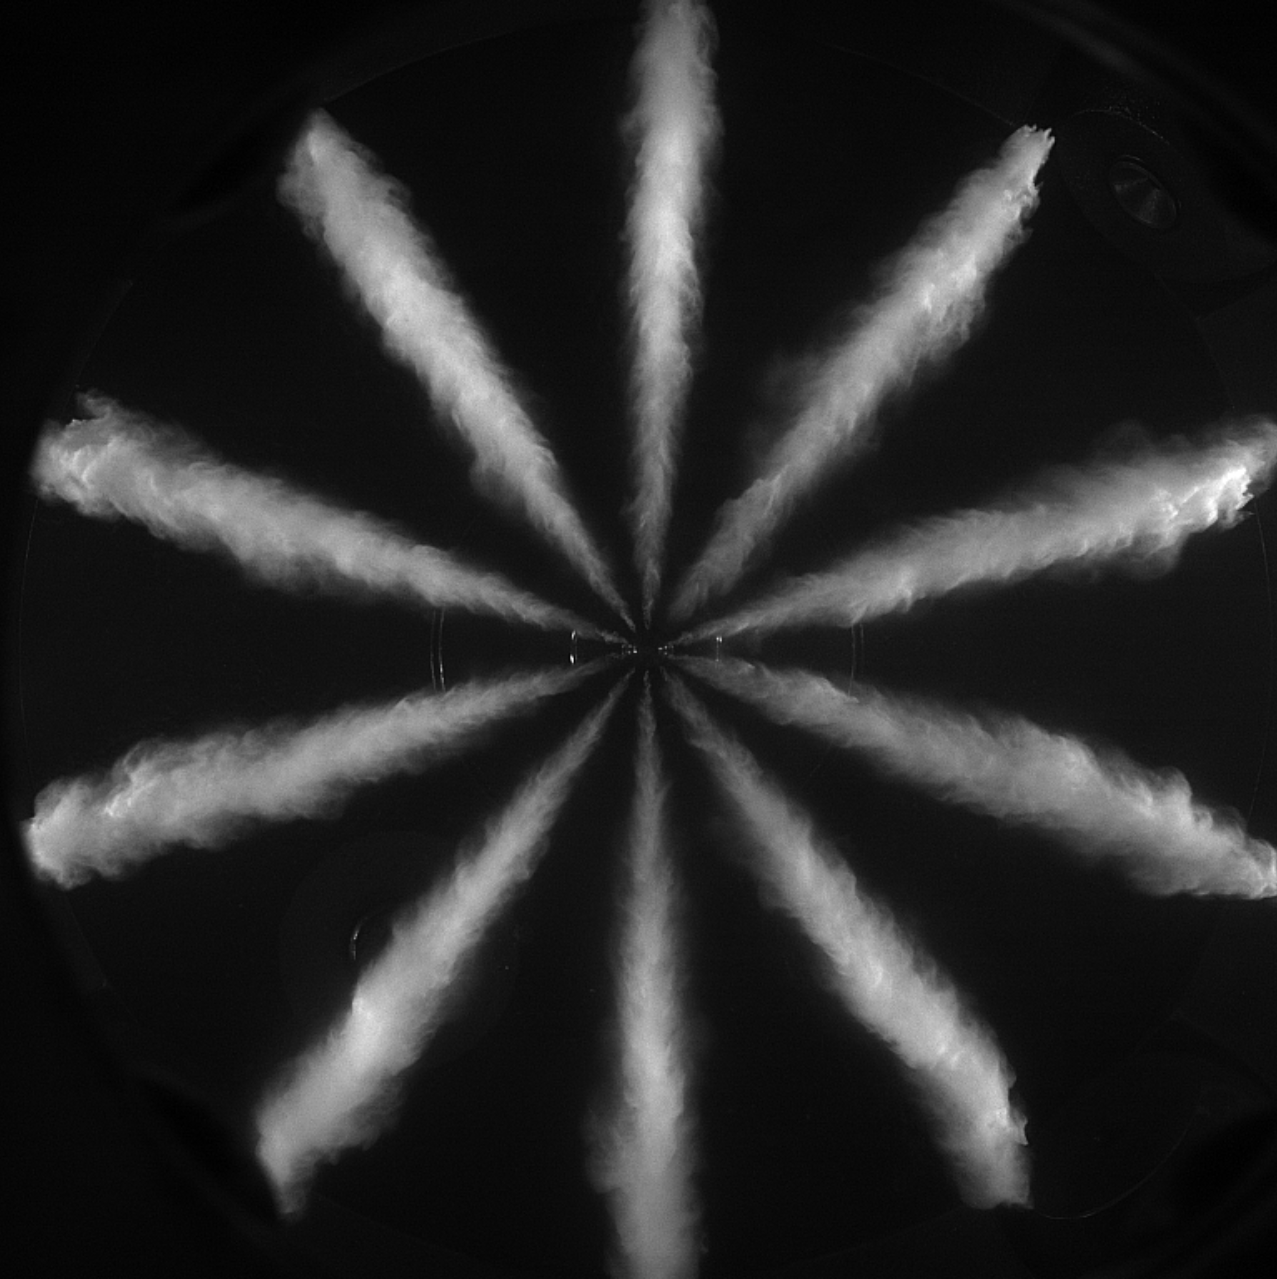
\includegraphics[width=0.9\linewidth]{../images/right_censoring_example.png}
\caption{Representative example of right-censoring in the spray images. Some plumes have already extended beyond the upper observation boundary and appear only as blurred ring-like edge traces near the limit, while other plumes are still fully contained within the visible window.}
\label{fig:right-censoring-example}
\end{figure}

This distinction has direct consequences for surrogate-model training. 
Treat a censored trajectory's visible endpoint as an ordinary regression label and the target is biased downward in exactly the region 
where long-range penetration should still be growing. 
The learner model is then encouraged to read the spray's exit from the image as physical saturation, which it is not. 
In practice, mixing censored and uncensored trajectories in the same training set under this setup produces unstable late-time gradients 
and an artificial flattening that propagates through every downstream prediction.

The reduced-order fitting stage in this thesis is therefore not introduced only as a smoothing device. 
It does double duty as a censoring-aware target-construction step. 
The fitted curve gives a compact and more stable representation of the trajectory, supports conservative extrapolation beyond the visible window, 
and dampens the sensitivity of downstream learning to the exact instant at which the optical trace becomes incomplete. 
The role is especially valuable for short pilot injections, 
where start-of-injection and end-of-injection transients already complicate the raw signal shape \cite{ZhouLiYi2021,ZhouLiLaiWei2019}.

\subsection{Multihole plume registration and symmetry exploitation}

Multihole injectors raise a problem that generic spray segmentation simply does not face. 
There is no single isolated jet to find. 
Instead, the image carries several plumes arranged around a common nozzle centre, 
with a known multiplicity and an approximately repeated angular structure. 
Multihole behaviour, importantly, is not just single-hole behaviour repeated \(N\) times: 
internal sac flow, hole-to-hole interaction, and plume-to-plume disturbances can shift the resulting spray morphology in ways that single-hole models 
do not anticipate \cite{JinKimKakamiNishidaOgataLuo2020,MopuriGrahnSedarskyHyvonen2024}. 
The computational task is therefore not just to detect spray pixels but to \emph{register} repeated plumes 
consistently across frames and operating conditions.

That is why the workflow moves from Cartesian image coordinates into nozzle-centred polar and plume-aligned coordinates. 
Once the spray is described on the angular axis, the repeated structure induced by the injector hole pattern becomes much easier to analyse: 
plume occupancy collapses to a one-dimensional periodic signal rather than fragmented edge content scattered across the image plane 
\cite{Szeliski2010Vision}. 
The subsequent use of harmonic analysis is then not a signal-processing trick reached for at random but a symmetry-exploiting registration rule 
--- the known injector multiplicity defines a natural angular frequency, and the phase of that harmonic gives rotational alignment for free 
\cite{CooleyTukey1965FFT}.

\subsection{Metric definition and boundary extraction in spray imaging}

Fuel-imaging literature is clear about a point that is easy to understate: 
the numerical definition of a spray metric is itself a modelling decision. 
Magnotti and Genzale showed that different liquid-penetration metrics can lead to materially different conclusions when validating diesel spray models, 
because different observables respond to different aspects of the underlying liquid distribution \cite{MagnottiGenzale2013}. 
The implication for Mie processing is important: a reported ``penetration'' value is not a universal truth but the output of a measurement rule 
applied to an optical signal --- change the rule, change the value.

The same caution applies to cone angle and boundary extraction. 
Johnson et al.\ showed that conventional threshold-based cone-angle estimation from back-scattered diesel images 
is sensitive to the chosen intensity threshold, 
and they proposed a profile-based alternative specifically to dampen that subjectivity \cite{JohnsonNaberLee2012}. 
The present work draws two lessons from that. 

First, it confirms that boundary metrics deserve to be treated as operational geometric descriptors, not as exact liquid-envelope measurements. 

Second, it argues for a cumulative-distribution penetration front and multiple boundary proxies, 
on the principle that a robust metric should rest on the bulk support of the plume rather than on one fragile leading pixel or one globally fixed threshold.

The result is a workflow that does not treat intensity processing as full physical-state recovery. 
It uses image-processing theory and prior spray-imaging evidence to construct reproducible, 
physically interpretable geometric observables and states their limitations explicitly, 
which is essential for a diagnostic whose outputs are method-dependent.

The Engine Combustion Network (ECN) benchmark work has documented the method-dependence of spray measurements in unusually systematic form. 
By testing nominally identical injectors (Spray~A and Spray~D) across multiple institutions, 
ECN found measurable inter-facility variation in liquid-penetration values, 
and concluded explicitly that optically measured liquid boundaries should be understood as quantities defined by a particular measurement protocol, 
not as absolute ground-truth representations of the liquid phase 
\cite{ecn_liquid_penetration,ecn_liquid_penetration_accessory,MeijerECN2012}. 
The experimental context here differs from ECN Spray~A (high-temperature, high-pressure evaporating conditions) and Spray~D (multihole nozzle) 
--- the present data come from a room-temperature pressurised chamber with a multihole marine nozzle and no fuel evaporation. 
The ECN methodological principle still applies: the numerical values of reported penetration and boundary metrics depend on the post-processing rules, 
and that dependency has to be visible when results are interpreted.

\subsection{Why deterministic, uncertainty-aware, and teacher-guided learning stages are all useful}

Data-driven surrogate models have established themselves as viable predictors of spray macroscopic characteristics in the recent literature. 
Neural-network approaches have been used to map operating-condition parameters directly to spray tip penetration and cone angle 
without paying the cost of a full CFD computation in between, with several studies reporting close agreement against reference penetration data \cite{VazKarathanasis2026,liu2020sprayreview}.
These results settle the question of whether neural networks are a feasible modelling layer for spray macroscopic properties 
--- they are. They do not, however, settle every question that matters here. 
Those studies typically assume complete, fully observable penetration trajectories as training labels 
and do not attempt to model inter-condition or inter-cycle uncertainty explicitly. 
The present problem is more restrictive on all three counts: 
short pilot-injection traces are dominated by SOI and EOI transients, 
the limited field of view turns a large fraction of trajectories into right-censored ones, 
and plume-to-plume and shot-to-shot variance is itself engineering-relevant information rather than an irreducible nuisance to average away. 
The learning framework here therefore takes the general data-driven spray surrogate as a starting point 
and adds three design elements aimed at those specific constraints: 
censoring-aware target construction, heteroscedastic uncertainty quantification, and a distillation-based refinement stage.

A deterministic multilayer perceptron is a reasonable first cut at a penetration surrogate 
because it can map a small set of operating-condition features and time to a continuous trajectory at modest cost \cite{BishopPRML2006}. 
In the baseline configuration, the network feeds on physically scaled inputs and is regularised by smoothness-related penalties on the trajectory shape.

The uncertainty-aware extension is motivated by something simpler than statistical taste: 
not all operating points and extracted trajectories deserve the same confidence. 
Heteroscedastic Gaussian negative log likelihood is the standard way to let a network predict both a mean and an input-dependent variance (i.e., providing an error bar width that varies with conditions for each operating point; see Section~\ref{sec:methods-terminology}) 
\cite{KendallGal2017}. 
In regression terms, this corresponds to the conditional model
\[
y=\mu(x,t)+\varepsilon(x,t),\qquad \varepsilon(x,t)\sim \mathcal{N}(0,\sigma^2(x,t)),
\]
which should be read here as a pragmatic statistical assumption rather than as a claim that the spray physics are literally Gaussian at every instant 
\cite{BishopPRML2006,KendallGal2017}. 
The present motivation is that the observed penetration spread is the aggregate effect of many unresolved factors: 
injector-hydraulic transients during pilot injection, sac and needle-opening dynamics near SOI, cycle-to-cycle differences in delivered momentum, 
synchronization offsets, and residual image-processing noise from the optical measurement chain. 
Zhou et al.\ already show that short-injection penetration behavior is strongly transient and regime-dependent near SOI \cite{ZhouLiYi2021}; 
in the current project, those unresolved perturbations are not modeled mechanistically one by one, 
so it is reasonable to treat their combined effect as an input-dependent residual distribution whose variance changes with operating condition and time. 
In this thesis the heteroscedastic stage is a completed modelling layer and teacher checkpoint, 
but not a final deployed product on its own; 
its value is realised together with the distillation and simplified screening stages.

The Gaussian assumption is not chosen only on grounds of physical realism 
--- it also pays for itself in the distillation stage. 
When both teacher and student outputs are represented as univariate Gaussians, the Kullback--Leibler divergence between them (measuring the information lost when using the student distribution to approximate the teacher distribution; a value of zero indicates the two distributions are identical) 
collapses to a closed analytical form:
\[
D_{\mathrm{KL}}\!\left(\mathcal{N}(\mu_1,\sigma_1^2)\,\|\,\mathcal{N}(\mu_2,\sigma_2^2)\right)
=\log\frac{\sigma_2}{\sigma_1}+\frac{\sigma_1^2+(\mu_1-\mu_2)^2}{2\sigma_2^2}-\frac{1}{2},
\]
which means the distillation loss can be evaluated exactly, with no Monte Carlo sampling and therefore no extra gradient variance injected into training. 
The direction of the divergence is a more delicate choice than its closed form suggests. 
Forward KL (student approximating teacher) is mean-seeking: 
it spreads probability mass broadly and tends to over-cover, which makes it conservative in the right way when late-time samples are sparse. 
Reverse KL is mode-seeking: it locks onto the teacher's dominant peak and is comparatively indifferent to thin outlier trajectories. 
In this application the two directions produce near-identical predictions in the operating range that matters, 
and forward KL was retained mainly because it is consistent with the negative log-likelihood objective already used in Stages 1 and 2 
\cite{BishopPRML2006,KendallGal2017}.
Recent work on knowledge distillation for regression under data scarcity has shown that teacher-soft targets can substantially 
reduce student prediction error precisely in regimes where direct labels are missing \cite{KangKang2024KDRegression} 
--- which is the regime this thesis lands in by construction.

A further refinement stage is justified once the supervision becomes uneven over time. 
Knowledge distillation was introduced as a way to transfer the predictive structure of a teacher network to a student 
by means of softer targets than hard labels \cite{HintonVinyalsDean2015}. 
Closely related teacher-student formulations are also used when supervision is limited or incomplete, 
because the teacher can provide a stable target signal in regions where direct labels are sparse, noisy, or absent \cite{TarvainenValpola2017}. 
In the present thesis, that logic is adapted to partially observed penetration trajectories: 
where uncensored raw observations remain trustworthy, they should directly refine the student; 
where the late-time raw signal becomes unreliable because of censoring and sample dropout, 
the teacher continuation is a more conservative guide than treating the disappearing tail as a hard physical label. 
This is why the third learning stage is methodologically different from simple fine-tuning: 
it combines direct raw supervision with teacher-guided regularization so that the model can improve early-time fidelity 
without being pulled downward by incomplete late-time observations.

\subsection{Spray--wall impingement mechanisms and probabilistic collision-risk screening}

Pilot-spray penetration control is first a combustion-organisation problem, not only a wall-avoidance problem. 
In dual-fuel diesel--gas engines, the geometric distribution of the pilot diesel spray 
--- including penetration, cone angle, and the liquid-phase envelope --- 
directly determines the spatial location and size of the ignition kernel, 
and thereby affects whether the flame can propagate efficiently into the premixed main-fuel gas charge 
\cite{Karim2015DualFuel,WeiGeng2016DualFuelReview,Sahoo2009DualFuelReview}. 
If the pilot penetration is too short, the ignition kernel may form in an unfavourable region or occupy too small a volume, 
which can weaken main-fuel flame propagation, increase unburned hydrocarbons such as methane slip, 
and reduce the overall combustion efficiency. 
If the pilot penetration is too long, even before clear wall contact occurs, 
it can also shift the relative placement of the ignition kernel and the gaseous charge, 
causing inefficient main-fuel burning and increasing the likelihood of liquid-wall contact \cite{WeiGeng2016DualFuelReview,Sahoo2009DualFuelReview}. 
Pilot penetration is therefore first a key control variable for main-fuel mixing, ignition-kernel placement, and combustion efficiency; 
on that basis, it is also the central geometric input for wall-risk screening. 
The penetration and uncertainty predictions developed in this thesis primarily support pilot-injection control and combustion-organisation assessment, while also supporting wall-risk ranking.

When that spatial control fails, liquid-phase spray contact with engine surfaces becomes one of the downstream consequences that must be managed. 
When liquid fuel reaches the piston crown or cylinder wall before evaporation or ignition has had time to consume it, 
a fuel film deposits on the surface, and the downstream consequences 
--- wall wetting, locally deteriorated mixing, elevated unburned-hydrocarbon emissions, and lubricant dilution 
--- are well documented across both passenger-car and heavy-duty contexts \cite{peraza2022swi,ahmad2025fueldilution,MorieiraMotaPanao2010}. 
The problem does not stay purely microscopic. 
Moreira \textit{et al.} are explicit in their review that single-droplet impact research has accumulated a sizable knowledge base, 
but extrapolating it directly to continuous spray impingement is a stretch: 
a spray plume behaves collectively, and that collective behavior is shaped by neighbour-droplet interactions, residual wall film, 
and secondary atomization phenomena that simply do not appear in isolated droplet experiments \cite{MorieiraMotaPanao2010}. 
The translation from droplet to plume is therefore a gap, not a smooth interpolation. 
The picture changes again at marine scale. 
The spatial scale of spray development in large-bore marine diesel engines is not a scaled-up version of an automotive case, 
and optical studies with full-size marine injectors confirm that wall confinement materially shifts both ignition delay and natural-luminosity 
flame intensity relative to a free-jet configuration \cite{liu2024marine_impingement}.

The simplest screening rule used in engineering practice has barely changed in two decades: 
compare the liquid-phase spray-tip penetration $S_\mathrm{tip}(t)$ against the nozzle-to-wall distance $L_\mathrm{wall}$, 
and flag impingement once $S_\mathrm{tip}(t) \geq L_\mathrm{wall}$ \cite{Baumgarten2006MixFormation}. 
Baumgarten's reference treatment of mixture formation in internal combustion engines codifies this practice, 
naming penetration correlations as the baseline trajectory descriptor and the penetration-to-wall-distance comparison 
as the default first-order impingement criterion \cite{Baumgarten2006MixFormation}. 
Two refinements of this idea are worth singling out. 
Park \textit{et al.}\ pushed the criterion further for high-pressure gasoline direct injection by reconstructing the radial fuel-mass distribution 
from spray images and combining it with injection-timing data to quantify the fuel-mass fraction actually striking the piston and cylinder wall; 
the trend they extract --- impingement falling as injection pressure rises and atomization sharpens --- is itself unsurprising, 
but the methodological contribution is more interesting: 
it shows that image-based analysis can deliver a quantitative impingement estimate without paying for a full CFD run \cite{Park2018WallImpingement}. 
Within the ECN framework, Peraza \textit{et al.}\ measured spray impingement on a controlled-temperature flat wall 
using a single-hole injector and characterized how the penetration-to-wall-distance relationship deforms with ambient density and temperature 
\cite{peraza2022swi}. 
Read together, the two studies confirm a single point: 
penetration depth, however it is measured, remains the load-bearing geometric input to any impingement screening worth taking seriously.

For short-pulse pilot injections, that deterministic threshold is too brittle as the primary screening tool. 
Penetration here carries non-negligible uncertainty from needle-valve transients, 
cycle-to-cycle fluctuations in delivered momentum, and residual optical-measurement noise, 
and the SOI/EOI-dominated regime makes steady-state correlations imprecise over a large fraction of the observable window. 
A binary pass/fail rule, applied on top of a quantity that is itself a distribution rather than a number, 
hides information that is useful for ranking candidate conditions. 
The framework proposed in this thesis therefore represents penetration as a conditional Gaussian distribution 
$S_\mathrm{tip}\sim\mathcal{N}(\mu(x,t),\,\sigma^2(x,t))$, 
and projects that distribution onto a two-dimensional engine-geometry plane centred on the nozzle. 
With the lateral spread modelled as a normal distribution governed by the spray half-cone angle, 
the spray probability density function takes the form of a rotated two-dimensional Gaussian. 
Under that simplified geometry, the collision-risk score is the probability-mass integral of this distribution over the cylinder-wall and piston-crown masks. 
The output should therefore be read as a probabilistic screening proxy, not as a validated production-grade impingement prediction.

\begin{table}[t]
\centering
\footnotesize
\setlength{\tabcolsep}{2pt}
\renewcommand{\arraystretch}{1.12}
\begin{tabular}{@{}L{0.20\linewidth}L{0.25\linewidth}L{0.25\linewidth}L{0.23\linewidth}@{}}
\toprule
Literature strand & What it supports & Remaining limitation for this thesis & Thesis response \\
\midrule
Mie optical diagnostics and geometric observables & Optical intensity can support penetration, cone angle, and boundary observables; ECN-style benchmarks confirm that optical metrics are method-dependent. & Intensity is not a direct liquid-volume-fraction or mass field, and penetration definitions change with downstream processing rules. & Treat outputs as optical liquid-envelope metrics with explicit boundaries and retain method-dependence caveats in the discussion. \\
Spray-penetration physics and short-pulse transients & Classical and transient penetration laws explain why penetration is physically meaningful and why it changes across injection stages. & Short pilot injections mix SOI, EOI, and injector-hardware time scales within the observable window, so one rigid correlation cannot cover the full trajectory. & Use flexible reduced-order targets and physically motivated scaling rather than one rigid law. \\
CUDA parallel image processing and multihole registration & Calibration, log preprocessing, gradients, polar mapping, Fourier registration, and robust fitting are established tools. & No single off-the-shelf method covers the full multihole video workflow, and single-jet segmentation tools do not reliably register repeated plumes. & Assemble an auditable pipeline from standard, inspectable operators and exploit symmetry through nozzle-centred polar and plume-aligned coordinates. \\
Data-driven surrogate modelling with censoring and uncertainty & ANN/MLP models can predict spray macroscopic quantities; censoring statistics, heteroscedastic regression, and teacher distillation are established tools. & Existing spray-surrogate work rarely treats field-of-view loss explicitly as right-censoring or makes input-dependent uncertainty a first-class output. & Integrate censoring-aware synthetic target construction, heteroscedastic NLL, and teacher-guided distillation within one learning framework. \\
Impingement-risk screening & Penetration-to-wall distance remains the central geometric input for first-order impingement screening. & Deterministic thresholds can hide the information needed for ranking under strongly transient, high-uncertainty conditions. & Output conditional Gaussian penetration predictions and project them onto simplified two-dimensional geometry to form a probabilistic impingement proxy. \\
\bottomrule
\end{tabular}
\caption{Synthesis of the reviewed literature and the corresponding design response in this thesis.}
\label{tab:literature-synthesis}
\end{table}

Pulled together, the existing literature provides the support strands summarised in Table~\ref{tab:literature-synthesis}. 
Mie scattering theory explains why optical intensity can only be converted cautiously into geometric observables. 
Computer vision and signal processing theory support the local steps of the image-processing chain, 
even though no ready-made tool covers the complete workflow. 
Diesel spray physics clarifies the meaning of penetration and cone angle as descriptors, 
and also clarifies the limits of what those descriptors can represent. 
ECN benchmark studies make the method-dependence of optical metrics explicit. 
Existing ANN/MLP surrogate studies show that fast regression of spray macroscopic quantities is feasible, 
but they do not naturally resolve the bias introduced by partially observed short-pulse trajectories. 
Spray-wall impingement literature confirms the central role of penetration as the geometric screening input, 
while exposing the fragility of deterministic thresholds under strongly transient, high-uncertainty conditions.

What remains unresolved is that no single strand treats the combined problem faced in this thesis: 
(1) SOI and EOI transients dominate the observable window in short-pulse pilot injection; 
(2) the finite field of view systematically right-censors the training targets; 
(3) multihole nozzles require registration and extraction procedures designed around plume geometry rather than single-hole tools applied after the fact; 
(4) the learning framework must integrate censoring-aware synthetic targets, heteroscedastic regression, 
and teacher distillation to avoid learning observation truncation as physical saturation; and 
(5) the predicted conditional Gaussian penetration must be mapped onto simplified engine-geometry masks 
to form a probabilistic risk proxy suitable for early design screening. 
The contribution of this thesis is not that it touches these five issues separately, 
but that it treats them as design constraints of one workflow. 
The following chapters test whether that integrated scheme holds together.

